\chapter{}
Nas férias, Tio Totó, o irmão mais velho do papai que morava na fazenda, vinha buscar as filhas na casa das tias, onde elas se hospedavam no período escolar.
De cambulhada, levava-nos a mim e ao Reginaldo para fazer companhia às primas.
Era uma alegria. 
Eu adorava a fazenda e até hoje minhas inclinações e preferências, em muitos aspectos da vida, têm suas raízes naqueles dias passados na Barrinha, na Pedra Branca e na Fazendinha. 

Tio Totó era um fazendeiro remanescente dos tempos em que o dono da terra era patrão, médico e juiz, com autoridade civil e criminal sobre seus colonos. 
De manhãzinha, a fila se formava na porta da cozinha e o atendimento começava: era conselho para um, sermão para outro, remédio para o filho daquele outro, curativo, injeção, encomendas para serem levadas mais tarde à cidade, conciliação das desavenças e por aí afora. 
Ao lado, silenciosa e atenta, Tia Albina, mulher, companheira e assistente, ia organizando a fila, desinfetando seringas, ajudando nos curativos, anotando os pedidos. 
A maioria era compadre, seja porque o casal lhes apadrinhara o casamento ou um dos filhos. Terminada a sessão, Tio Totó tomava mais um cafezinho na beira do fogão e saía para a roça. 
Quase nunca se dando ao trabalho de abrir a porteira. 
Preferia por as mãos sobre o mourão da cerca e agilmente pular sobre o arame, vigoroso e elástico. 
Tínhamos por ele o maior respeito, senão medo, que a Tia Albina cuidava de alimentar: \textit{``-- Olhe que quando o Totó chegar, o pau vai comer!''}. Era água na fervura.
Porque o tio era bruto e quando ficava bravo não media nem palavras, nem gestos. 
Num prenúncio aterrador do que estava por vir, seu olho estrábico metia-se de tal forma para dentro que só lhe víamos o branco da esclerótica. 
Mas, também sabia ser divertido e nos levava a passear na sua caminhonete, recolher prendas nas fazendas vizinhas para a quermesse do padre, ou tomar sorvete na cidadezinha próxima, sua amada Boa Esperança. 
Pela vida inteira, até morrer, Boa Esperança, sua terra natal, ocupou o centro das suas preocupações, sobrepondo-se a quaisquer outras, incluídos aí mulher, filhos e negócios. 
Nunca desistiu de colocar sua cidade no mapa do desenvolvimento paulista e para tanto se elegeu prefeito por duas vezes e vereador outras tantas. 
Os conchavos políticos eram realizados ali mesmo no terreiro e com uma característica \textit{sui generis}: os participantes eram obrigados a ficar de cócoras porque seu líder, meu tio, preferia essa posição para, didaticamente, expor suas estratégias, desenhando-as com um graveto na poeira do chão.

\begin{figure}[H]
\centering
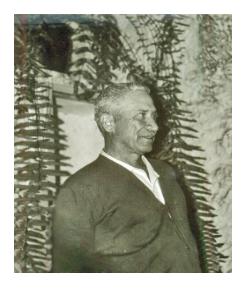
\includegraphics[width = 0.6\linewidth]{8/tio-totó.png}
\caption{Tio Totó.}
\end{figure}

Tia Albina trazia em si toda a sabedoria intuitiva e matreira da nossa gente cabocla. 
Ainda que usualmente se mantivesse quieta e passiva à retaguarda do companheiro, tinha uma luz própria que só percebia quem lhe ouvisse as observações cochichadas por entre o riso silencioso e sacudido. 
Que observadora implacável era ela! Nada lhe escapava.  
Gordinha, baixinha, sabia, contudo, irradiar majestade quando andava entre seus súditos na colônia. 
Sem nem levantar a voz.  
Vestidos invariavelmente ``ramadinhos'', como ela gostava, avental e chinelinhas, cabelo preso em coque na nuca, mal raiava o dia e lá estava ela no comando das tarefas domésticas, pois que seu amo e senhor queria tudo a tempo e a hora, embora fosse ele próprio completamente imprevisível, a ponto de que, na família, ``totozão'' virou epíteto para os eternamente fora de hora.  
O tio não tinha hora para coisa alguma e podia aparecer com um bando de correligionários ou amigos para almoçar sem nenhum aviso prévio. 
Disso resultou que ninguém, como Tia Albina, desenvolveu tamanha competência em produzir refeições saborosas em tempo recorde. Havia uma janelinha estratégica na cozinha, de onde se via a estrada da fazenda. 
Assim que divisava um carro diferente acompanhando o do tio, Tia Albina saia porta afora, agarrava certeira o primeiro frango que lhe passasse na frente e quando a visita sentava para conversar, já o aroma do seu insuperável franguinho frito inundava a casa toda. 
Mais uma corridinha à horta e o banquete estava pronto! Com a carinha mais sossegada do mundo, ela sorria aos elogios:
\textit{``-- Que nada''}, dizia, \textit{``comidinha simples da roça. Aposto que na cidade vocês comem coisa muito melhor''}.

\begin{figure}[H]
\centering
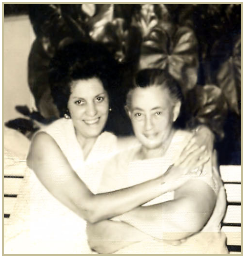
\includegraphics[width = 0.6\linewidth]{8/tia-albina.png}
\caption{Tia Albina abraçada por mamãe.}
\end{figure}

Muitas vezes me ocorreu que minhas primas perderam muito por não terem sido criadas pela mãe.
A mais velha foi-lhe tirada muito cedo e entregue à avó Teresa.
Parece que era outro costume trazido da Itália, o de levar os primogênitos para serem educados na casa dos avós paternos.
Em casa, a tradição foi derrotada pela resistência feroz e intransponível da minha mãe.
Ainda bem.
Tia Albina, porém, curvou-se à vontade do marido.
Aos poucos, as outras três lhe foram sendo tomadas quando chegavam à idade de freqüentar a escola.
Só lhe deixaram o temporão, Reginaldo Antônio, que contrariando os prognósticos de que criado na roça nunca seria alguém, é hoje um bem sucedido homem de negócios e um ser humano por quem tenho carinho e muita admiração.
Se mágoa restou em minha tia pelas filhas que lhe foram subtraídas, nunca demonstrou.
Mas acho que teria sido, sob muitos aspectos, uma mãe intuitivamente criativa.
Ensinou-nos a brincar com sucata, boizinhos de bucha, a fazer carrinhos de carretéis vazios.
Com caquinhos de louça nos fez imaginar ricas baixelas nas brincadeiras de casinha.
Com ela, aprendemos a fazer bruxinhas de pano, recortar figuras de moças e rapazes de revistas velhas para representar histórias que nos distraiam por horas seguidas.
De outras vezes, riscava flores ingênuas em pedaços de sacos alvejados e nos ensinava a bordar com linhas coloridas.
Prontos os bordados, ela fazia bicos de crochê à volta, transformando-os em toalhinhas que fazia questão de engomar para com elas enfeitar toda a casa.
Franqueava-nos também um maravilhoso baú onde guardava sapatos e vestidos antigos e nos dava, para acompanhar, sobras de pó de arroz \textit{Lady}, \textit{``rouge''} e toquinhos de batom.
Divertia-se vendo-nos encarnar madames, atrizes e princesas, convencidas de que estávamos deslumbrantes! Do bolso do avental.
sacava inesgotáveis moedinhas com que corríamos para comprar pirulitos, suspiros e ladrilhos de goiabada na vendinha do povoado.
E quando fazia pão, punha-nos à volta da mesa e nos dava pedaços de massa para que cada um fizesse seu próprio pãozinho, com a forma que a imaginação sugerisse.
Depois, punha-os para assar e os comíamos no lanche com queijo caseiro derretido na brasa.


Da casa da Tia Albina íamos com frequência para a da Tia Yolanda, que sempre morou não muito longe da cunhada e com ela dividia a tarefa de nos receber nas férias.
Já esta outra tia, a ama e senhora primeiro da Barrinha e depois da Fazendinha, como boa Filpi, tinha o gênio instável da raça.
Adorava crianças.
Cozinhava divinamente, empanturrava-nos de doces e bolinhos até a náusea.
Divertia-se com nossas traquinagens, mas nunca sabíamos quando sua braveza viria à tona, o que nos punha um tanto ressabiados.
Diziam que ela era a mais brava das irmãs.
Durante o tempo em que moramos, Reginaldo, mamãe e eu na casa dela na Barrinha, Reginaldo, que era muito levado, andou experimentando aqui e ali amostras do seu famoso temperamento.
Já eu não me lembro de lhe ter ouvido uma palavra mais áspera.
Nem mesmo quando ela encontrou as preciosas botas de montaria do seu Tio Aniello entupidas de massa crua, fermentada e embolorada.
Tio Aniello era meio parente do Vô Reginaldo, um senhor muito elegante e educado, casado com uma francesa e que vinha anualmente à fazenda para caçar codornas.
Brincando no quarto dos arreios, achei que as botas dele davam um ótimo forno para assar o pão das minhas bonecas e acabei esquecendo tudo lá, apodrecendo por dias e dias.

Tia Yolanda não teve filhos.
Talvez por isso tivesse menos jeito que a Tia Albina para lidar com os sobrinhos.
Ou talvez tivesse menos motivos para ser feliz.
Entre as irmãs, ela teve a educação mais cuidada.
Como era a filha mais velha, viveu a adolescência nos tempos de prosperidade do Vovô.
E, para aprimorar sua educação, chegou a morar por algum tempo com um irmão da Vó Teresa, um tal Tio João, muito abastado, casado com uma professora de maneiras refinadas que ensinou à Tia Yolanda modos e gostos de madame.
E minha tia era vocacionada para a coisa.
Atestava-o gesto característico de erguer delicadamente o indicador e o mindinho junto à face, quando se punha a contar um caso.
Porém Tio Zé, o marido, nunca deu muita sorte na vida.
Na verdade, nada do que lhe era confiado ia adiante.
Imagino até que teriam passado dificuldades se não morassem no campo que lhes provia as necessidades mais básicas.
Hoje, relembrando as sedes simples de ambas as fazendas, dou-me conta da quase penúria em que viviam.
O enxoval era de algodãozinho alvejado, áspero e imaculadamente branco.
Igualmente brancas eram as capas do sofá improvisado e das poltronas.
Com bicos de crochê e bordados, ela disfarçava a pobreza tecido.
Mas era a limpeza o grande trunfo e o grande luxo daquela decoração franciscana.
Meu Deus, como Tia Yolanda se devotou à limpeza, pela vida toda! Ainda que Os Filpi e os Vitta parecessem disputar o campeonato mundial do asseio doméstico, ninguém, para mim, batia Tia Yolanda na competência de fazer emanar das roupas, da casa, das louças, da mobília, aquele aroma inesquecível de água pura, de sol, de limpeza.
Ambas aquelas moradas humildes, a da Barrinha e a da Fazendinha, sempre produziram em mim o mesmo efeito de paz e integração com a vida.
No silêncio da tarde, o perfume das flores simples, do pé de jasmim, do capim-cidreira, da moita de arruda, trazido pelo vento que entrava pelas janelas fazendo esvoaçar as cortinas alvas, envolvia-me numa sensação de felicidade e completude que pelo resto da vida eu tento debalde reconstituir nas casas onde moro.
Faltam-me, entretanto, as grandes vascas de lavar roupa que a tia emoldurava de rosinhas trepadeiras e os varais batidos de luz onde os lençóis e toalhas panejavam contra o céu, o branco azulado de anil quase cegando a gente.
Faltam-me também suas mãos hábeis e fortes, contidas e suavizadas pelas maneiras fidalgas, lavando, esfregando, fervendo, areando, engomando, eternamente, incansavelmente.

\begin{figure}[H]
\centering
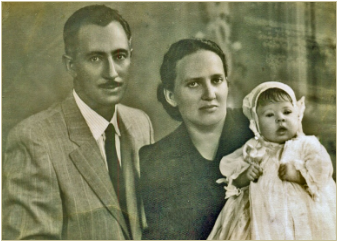
\includegraphics[width = 0.8\linewidth]{8/zé+yolanda.png}
\caption{Tio Zé e Tia Yolanda com minha prima Laura.}
\end{figure}

Essa atmosfera meio rural que leva as pessoas a acharem que as casas que eu arrumo têm um jeito de fazenda ou de casa de avó, devo-a às lembranças que ficaram desses lugares da minha infância.
Da nostalgia daquela estética ingênua das paredes brancas, do chão de tijolo e tábuas lavadas, das toalhinhas de crochê, dos canteiros de Maria-sem-vergonha, das cercas e portões enroscados de melindro e flor-de-São-João.
Mas, não seria justo deixar de mencionar a contribuição que me veio, também intensa, da casa das tias, irmãs do meu pai e da minha avó Didi, porque nelas eu andava quase diariamente e ambas, ainda que urbanas, conservavam o mesmo frescor singelo, a honesta simplicidade que tanto me encantava naquelas outras, as dos tios da fazenda.


A casa da Vó Didi, a primeira de que me lembro antes que Tia Maria Angelina se tornasse moça e começasse a impor seu gosto moderno e mais sofisticado, acachapava-se, baixinha e esparramada, numa esquina do Largo da Câmara.
Era daquelas de janela na rua, típica construção popular de inspiração portuguesa, tão comum nas antigas cidades brasileiras.
De precioso só mesmo a imensa mangueira que sombreava os fundos do grande quintal e o jardim lateral, o ``ai-Jesus'' da vovó, onde se misturavam em deliciosa confusão flores, folhagens, hortaliças, legumes, ervas de tempero e mezinhas.
Dentro, nada de sofás ou tapetes.
Motivo de orgulho eram a sala de jantar completa, a cômoda e dois criados-mudos de jacarandá cheiroso e finamente entalhado, fabricados na Mobiliadora do Tio José.
As panelas brilhavam como prata polida.
Assim como o chão encerado de joelhos e lustrado no escovão.
O cheiro que vinha do fogão à lenha era, segundo meu pai, tal como o sabor que ele prenunciava, inimitável.
Até hoje, nenhuma de nós, descendentes, conseguiu reproduzir nem um, nem outro, embora os ingredientes fossem pobres e a comida feita às pressas, entre uma e outra das muitas atividades da atribulada Didi
Para o molho de macarrão, exigente em calma e capricho, de bom grado ela passava o bastão ao marido, que ela não tinha tempo e nem paciência para tanta firula.

\begin{figure}[H]
\centering
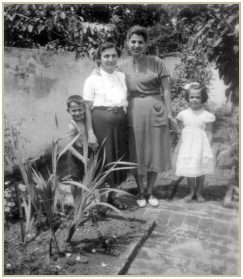
\includegraphics[width = 0.6\linewidth]{8/no-jardim.png}
\caption{No jardim da casa da Vó Didi.}
\end{figure}

Já a casa das tias, na Avenida D.Pedro II, embora externamente aparentasse certa elegância citadina com suas janelas altas e o porão que lhe elevava o pé direito, internamente parecia e funcionava como uma casa de fazenda.
A grande copa de assoalho lavado era o coração da residência.
Ali se passava roupa, faziam-se os trabalhos de agulha e recebiam-se as visitas dos mais chegados para o cafezinho coado sempre em duas versões: uma mais forte para os homens que o tomavam puro e outra mais fraca, para comer com bolos ou biscoitos, para as mulheres.
Vó Tereza, enquanto viveu, sentava-se rente à porta que abria para a cozinha.
Dali tinha um olho nas panelas que a Tia Glória ajudava a administrar e outro na engomação das roupas ou no cerzido das meias, o crochê, o bordado e a costura, a cargo da Tia Neta ou da Tia Imaculada.
Dos cercados do quintal vinham o frango, a galinha gorda, mortos e depenados na hora, os ovos frescos, o leitãozinho e, perto do Natal, até o cabrito.
E, da horta, o tomate, as verduras e temperos.
Pouco frequentávamos a sala de visitas.
Era vedada às crianças, sempre fechada, só aberta para a limpeza diária e para as visitas de cerimônia, pois guardava o que sobrou dos tempos de fausto do café: porcelanas, cristais e o grande piano alemão que ainda ostentava os castiçais de bronze fixados de cada lado do suporte para partituras.
Mas, dos quartos, dos lençóis brancos e dos travesseiros em que nos aninhávamos nas noites de festa, quando o sono nos vencia, emanava aquele mesmo cheiro de sol e água pura que me transportava, nos sonhos, de volta para a Barrinha, para a Fazendinha, para a Pedra Branca.

\begin{figure}[H]
\centering
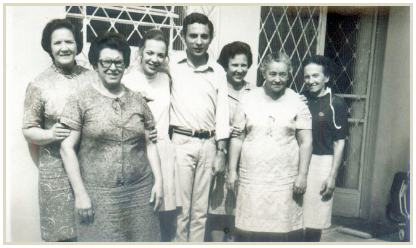
\includegraphics[width = 0.8\linewidth]{8/tias-no-noivado.png}
\caption{Ladeando Paulo e a mim, a partir da esquerda, as tias Glória, Imaculada, Antonieta, Albina e Yolanda, no dia do nosso noivado.}
\end{figure}

Essas mulheres da minha infância, tias e avós, suas casas, os perfumes que evolavam dos seus fogões, das suas hortas e jardins, dos assoalhos lavados, dos lençóis e toalhas que me envolviam, a quietude mansa que espalhavam ao seu redor quando, findo o trabalho do dia, sentavam-se para bordar, costurar, crochetar, alimentavam em mim a crença mágica de que detinham o poder de pôr em harmonia todo o Universo.
De noite, quando deitava minha cabeça naqueles travesseiros recheados de paina cheirosa que elas pacientemente descaroçavam e desfiavam, invadia-me a certeza tranquilizadora de que não só a casa, mas o mundo todo estava limpo e arrumado, na mais absoluta paz.
Então, eu me abandonava ao sono, confiante e feliz.
Se hoje, mesmo sob protestos, tento conservar as tradições que delas me vieram, é com certeza na ilusão de reeditar um pouco desse feitiço para os que não tiveram a sorte de experimentá-lo.
